
 \documentclass[letterpaper]{article}
\usepackage{underscore}
\usepackage[left=2.0cm, right=2.0cm, top=2.0cm]{geometry}
\usepackage[utf8]{inputenc}
\usepackage{graphicx}
\usepackage{graphics}
\usepackage[spanish]{babel}
\usepackage{lipsum}
\usepackage{float}
\usepackage{subfigure}
\usepackage{biblatex}
\usepackage{csquotes}
\usepackage{color}
\title{\textbf{Brazo Programable de Fácil Uso }} 

%plantillas de comandos 
%subrrayado con color de texto    \colorbox{blue}{\textcolor{white}{caca de la vaxa}}
\author{Ledesma Hernández Miguel Ángel, Carrasco Quiñones Karla Daniela, Reyna Gurrola Marcela\\ y Alcantar Díaz Joel Alejandro.}
\date{20/09/2019}
\begin{document}
\maketitle
\begin{center}
    
\includegraphics[scale=0.5]{Img/UPZMGlog.png}\\
    \vspace{1cm}
    Universidad Politécnica de la Zona Metropolitana de Guadalajara.\\
    \vspace{1cm}
Ing. en Mecatrónica.
\end{center}\newpage
\begin{large}
    \begin{LARGE}
        \textbf{Planteamiento del problema.}\\
    \end{LARGE}%hola bebe
    \begin{large}
    En la actualidad las máquinas estan presentes en cualquier empresa que se pueda considerar autónoma a pesar de la complejidad en la programación de las mismas, esto lleva a muchas empresas emergentes e incluso ya consolidas a no comprarlas por el coste que conlleva un equipo de estos y el temor a no poder usarlas correctamente por falta de personal capacitado para operar las mismas en la empresa. Esto crea problemas ecnómico, ya que no se aprovecha el óptimo funcionamiento de la maquinaria.\\
    De esto lo mas importante sería la programación del equipo para poder operar el mismo. Esto es mas que nada debido a la poca importancia que en México se le da a automatizar una fábrica, por poner un ejemplo, y el capital económico que esta dispuesto a invertir en la capacitación de sus empleados.\\
    Es por eso que una unidad que se pueda programar solamente moviendo un similar a escala o del tamaño que se requiera podría sustituir la programación en muchos casos y facilitar el uso de estas unidades.\\
    \end{large}
\end{large}

\begin{large}
    \begin{LARGE}
       \textbf{Formular el problema.}\\
    \end{LARGE}
    
    ¿Es cara una de estas máquinas?\\
    Ciertamente su coste sería un poco mas elevado que el de una máquina normal pero la facilidad que brindaría al usuario sería superior a un brazo mecánico común.\\
    %Esta parte no se si va aquí.

    ¿Es complicado utilizar una de estas máquinas?\\
    En lo absoluto, la capacitación necesaria para la operación del brazo sería minima dada la capacidad que tendra de memorizar los movimientos que el operador haga con él.\\
    
    
\end{large}

\begin{large}
    \begin{LARGE}
        \textbf{Objetivo general.}\\
       
       
        ¿A dónde queremos llegar?\\
     
         
    \end{LARGE}
        Se quiere crear un brazo mecánico que pueda ser manejable por cualquier persona, siendo así fácil de programar con una GUI[Graphic User Interface]. El coste no cuenta únicamente con el hardware, si no con el trabajo de los desarrolladores y el futuro ingreso por parte de la empresa que solicite el objeto puesto que de no tener un simple GUI requerirá de la contratación de un experto que púeda manipular correctamente la máquina.\\
 \vspace{.6cm}
        \begin{figure}[htbp]
            \centering
            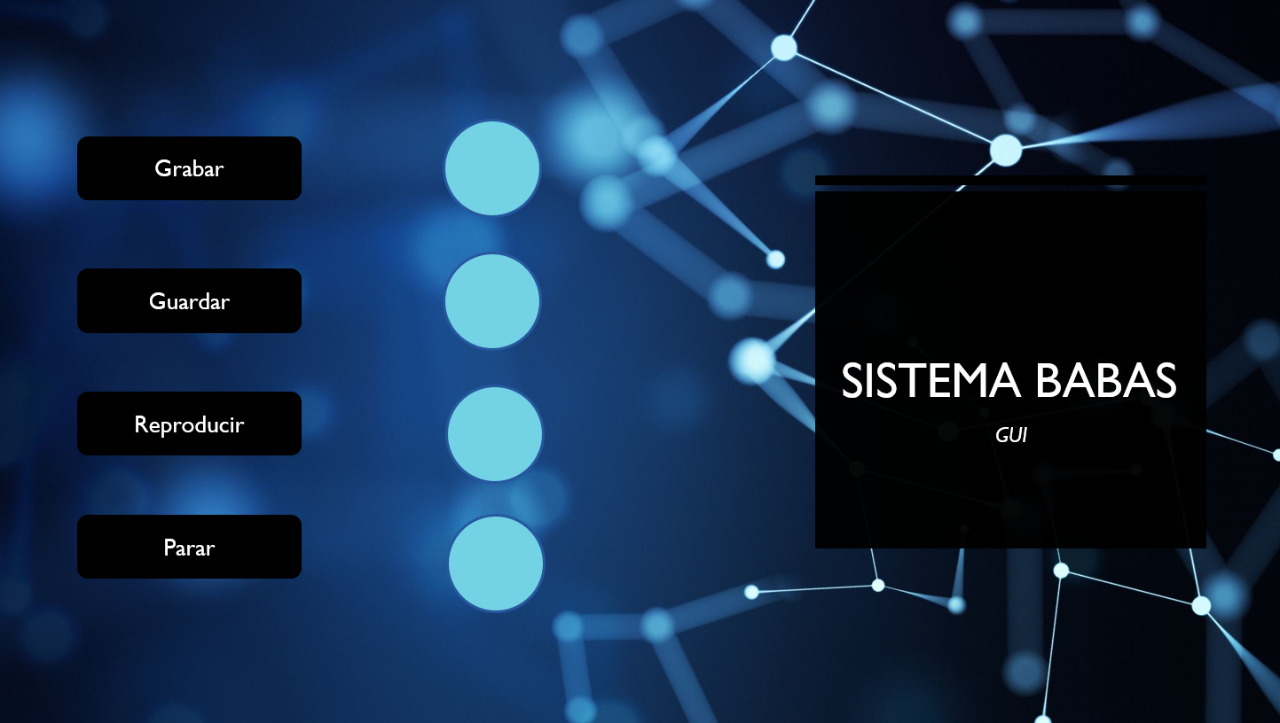
\includegraphics[scale=0.2]{Img/babas.jpeg}
            \caption{GUI}
            \label{fig:gui}
        \end{figure}\\
    Dentro de esta interfaz gráfica el usuario podra guardar los datos del movimiento del sistema robótico para despúes reproducirlos o crear un espectro calculado de los movimientos que hace [esto es útil para generar documentos con las coordenadas y la cantidad de voltaje que debe pasar por el circuito] para poder simular este movimiento en otros sistemas de la misma categoría. \\
    Queremos que el sistema sea accesible para todos los usuarios y que sea rentable por costos además de funcionamiento. Las aplicaciónes dependerán de la necesidad del usuario. Esto por la adaptabilidad de el brazo[Puede cambiar las puntas para tener distintas funciones], como ejemplo una pinza de punta fina y otra de punta más gruesa.\\
    Queremos que los costos no sean elevados tanto en software[un sistema sencillo] como en hardware  para que este sistema pueda ser implementado inclusive como método de aprendizaje en alguna institución o en el uso para análisis de circuitos eléctricos y electrónicos.\\\\
        
\end{large}

\begin{large}
    \begin{LARGE}
        \textbf{Objetivos del proyecto.}\\
    \end{LARGE}
    \begin{enumerate} 
        \item Recopilar la información necesaria para la creación del proyecto.
        \item Estudiar la información recabada.
        \item Seleccionar la información mas reelevante que se encontró.
        \item \colorbox{cyan}{Identificar los componentes necesarios para la contrucción del brazo a escala.} 
        \item Elaborar una lista de precios del material.
        \item Seleccionar los componentes que mas se ajusten al presupuesto.
        \item Comprar los componentes.
        \item Determinar los grados de movimiento del brazo.
        \item \colorbox{cyan}{Iniciar el armado del primer prototipo.}
        \item Idear un marco de pruebas para el prototipo.
        \item Realizar las pruebas necesarias.
        \item \colorbox{cyan}{Corregir los problemas que puedan presentarse.}
        \item Que el brazo levante 1kg como mínimo.
        \item \colorbox{cyan}{Crear una fuente conmutada especialmente para el brazo.}
        \item \colorbox{cyan}{Crear PCB específicas para el brazo}
    \end{enumerate}
    %no escuho si me neeitan me escriben abajo de obj generales para escribir bien xd
\end{large}
\vspace{1.5cm}
\begin{large}
    \begin{LARGE}
        \textbf{Justificación.}\\
    \end{LARGE}
    %aquí tienes que poner el texto de la justificación
    % usa este comando si quieres poner un texto remarcado en azúl \colorbox{blue}{\textcolor{white}{caca de la vaxa}}
Este proyecto permitirá programar los movimientos del brazo robótico mediante una técnica espejo, lo cual evita es uso de comandos y fallas al momento de compilar el programa. Además, cualquier persona que cuente con los conociminetos básicos sobre cómo guardar los movimientos del robot podrá usarlo y programarlo para cualquier cosa que desée. 
\end{large}
\vspace{1.8cm}\\
\begin{large}
    \begin{LARGE}
        \textbf{Delimitación.}\\
    \end{LARGE}
  El enfoque que queremos realizar en este proyecto es realizar un brazo robótico funcionable, que nos permita comprender el uso de este conforme a otras materias que tenemos, también queremos que nuestro brazo realice movimientos indispensables y factibles para el uso de empresas o para que los futuros alumnos de la UPZMG tengan con que practicar y comprender el mecanismo y movimiento de dicho brazo.\\\\
  Por el momento el brazo al ser un prototipo de la funcionalidad solo podra levantar 1kg máximo como demostración de las capacidades de lectura de los sensores, también una limitante es el material ya que sera contruido con MDF y el control que puede tener el usuario. Además de contar con unas medidas de 40cm de ancho, 40cm de largo y 50cm de alto aproximadamente. 
\end{large}

\begin{large}
    \begin{LARGE}
        \textbf{Matriz de roles.}\\
        
    \end{LARGE}
    

%\begin{table}[]
\begin{tabular}{|c|c|c|c|c|}
\hline
    Actividades & Joel & Miguel & Marcela & Karla     \\ \hline
    Investigar sobre el desarrollo y      & R & R & R & R\\   
    en que nos puede ayudar             &   &   &   &  
     \\ \hline
    Cotizamos el coto de los materiales & E & E & E & E \\
    requeridos para la realización de   &   &   &   &   \\
    nuestro brazo                       &   &   &   &   \\ \hline
    Compramos los usos de los componentes que requerimos & N & N & N & N \\
    para la realización de nuestro brazo.                &   &   &   &   \\ \hline
    Realizamos el primer prototipo para saber si nuestro & N & N & N & N \\
    proyecto cometa errores y arreglarlos, asi como saber &  &   &   &   \\
     si esto esta en funcionamiento.                     &   &   &   &   \\ \hline
    Haremos pruebas con nuestro brazo para\\ tener en cuenta nuestros errores.   &  N   &  N  &  N  &  N \\ \hline
    En este tiempo nos encargaremos de repa-\\ rar los errores que tengamos con nuestro\\ brazo. &  N  &   N  &   N   &  N \\\hline
 
\end{tabular}
\end{large}\\ \newpage

 
   
   
   \begin{LARGE}
   \begin{figure}[htbp]
        \textbf{Diagrama de GANTT.}\\
       \includegraphics[scale=0.5]{Img/gantt2.png}
 \end{figure}
   \end{LARGE}
   \newpage
   \begin{large}
       \begin{large}
       \textbf{Matríz de materiales y costos.}
           \begin{table}[htbp]
\begin{tabular}{|l|l|l|l|} 
\hline
Producto      & Costos         & Modelo               & ¿Qué es?                               \\ \hline
Motor a pasos & 50 pesos       & 28byj-48             & Un motor programable                   \\ \hline
Raspberry     & 780 pesos      & p3                   & Una pequeña computadora tamaño tarjeta \\ \hline
Cables varios & 50c c/u        & cupper               & Utilidad de conec                      \\ \hline
Resistencias  & 50c c/u        & Null                 & Resistores para el flujo de corriente  \\ \hline
Impresión 3d  & X pesos        & Null                 & Impresiones varias                     \\ \hline
Tubos PVC     & 30 pesos metro & 1/2                  & Soportes del braso                     \\ \hline
Estaño/cautín & 150 pesos      & generico             & Para soldar                            \\ \hline
Placa de base & X pesos        & depende del material & Donde se montará                       \\ \hline
Buzzer        & 25 pesos       & Null                 & Para el sonido                         \\ \hline
Leds          & 10 pesos c/u   & Null                 & Estilizar el modelo                     \\ \hline
Giroscopio    & 50 Pesos       & MPU6050              & Modulo de giroscopio y acelerometro    \\ \hline
Potenciometro & 6 pesos c/u    & Null                 & Resistencia variable de 10k            \\ \hline
\end{tabular}
\end{table}
       \end{large}
   \end{large}
\\\\
\begin{large}
\textbf{Funcionamiento teorico.}\\\\
El brazo funciona a travez de la captación de movimientos en un sistema controlado por una mano humana. Este captará los movimientos para después traducirlos y enviarlos, el proceso cuenta de variables con mismos valores actualizandose constantemente con el valor de el anterior, como ejemplo de esto se encuentra u y $u'$, donde u=5 y $u'$=10, dentro de un código programado no se debe poner el caracter reservado de $" ' "$ pero se pone un identificador para el captador y para el emisor, dentro de este programa se hará el proceso de captación de u para después traducir y mandar señales a $u'$ teniendo como base un registro guardado de sus coordenadas relativas y/o absolutas dentro de un plano cartesiano lógico ubicado sobre el sistema. \\
Tomará cada motor como un sistema individual que en conjución con los demás hará un sistema complejo de agarre de pinza y movimiento. El agarre de pinza constará de dos estados, uno en el que la mano del usuario esté abierta(Estado1) y una donde la mano esté cerrada(Estado0), siendo posible escalar el proyecto para la detección exacta de la posición, reduciendo de dos estados a uno que traduzca la posición real del servomotor del usuario para replicar lo mismo en el sistema.
\\
\end{large}
\newpage
\begin{large}
\textbf{Explicación de la aportación  de cada materia cursada en el cuatrimestre al proyecto}


\begin{table}[htbp]
    \centering
   
   
    \begin{tabular}{|l|l|}
    \hline
Materias de 4to  &  Detalles de aportación al proyecto 
                        \\ \hline
Inglés & El inglés es necesario para programar y\\
        & leer la gran mayoría de información\\
        & disponible en internet.
                        \\ \hline
Ética profesional & Aporta el ser consientes de que esta máquina \\
                  & no se hace con la intención de sustituir al ser\\
                  & humano, si no con la inteción de facilitar su\\ 
                  & trabajo y evitar accidentes. 
                        \\\hline
Estructura y propiedades de los materiales & La selección de un material\\
                                 & resistente pero flexible como la\\
                                 & medera, ademas del tipo de adhesivo\\
                                 & que se utilizará.
                        \\\hline
Programación de periféricos & Para que el brazo se capaz de guardar\\
                            & los movimientos se necesita programarlo\\
                            & para lograr crear un interfaz más\\
                            & gráfica y amigable con el usuario.
                        \\\hline
Sistemas electrónicos de interfaz & La fuente que alimentará el brazo\\
                                 & deberá contar con los valores de\\
                                 & voltaje y corriente necesarios para\\
                                 & mantenerlo en óptimo funcionamiento.
                        \\\hline
Controladores lógicos programables & El funcionamieto principal del\\
                                &brazo se llevará a cabo gracias a una\\
                                & tarjeta que mediará los grados de\\
                                & movimiento del los servo-motores.\\
                                \hline
        
    \end{tabular}
\end{table}

\end{large}
\newpage
\begin{large}
\textbf{Boceto preliminar}
  \begin{figure}[htbp]
            \centering
            \subfigure[Modelado preliminar]{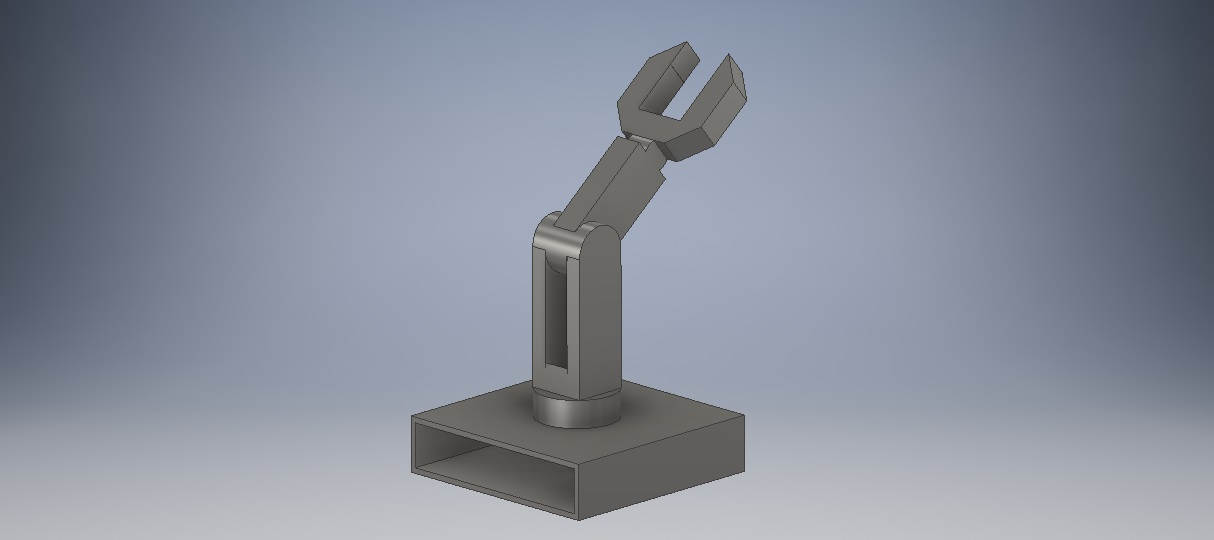
\includegraphics[scale=0.4]{Img/Brazo.jpg}}
            \subfigure[Medidas aproximadas y dibujo en mm]{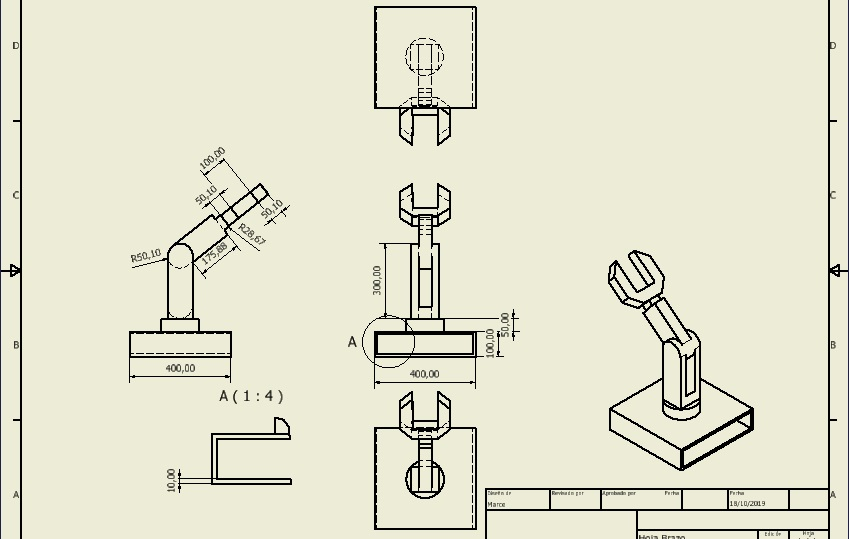
\includegraphics[scale=0.6]{Img/Hojabrazo.jpg}}
            \caption{Primer boceto del brazo}
            \label{fig:bra}
        \end{figure}
      
        
 
  %\begin{figure}[htbp]
   %         \centering
    %        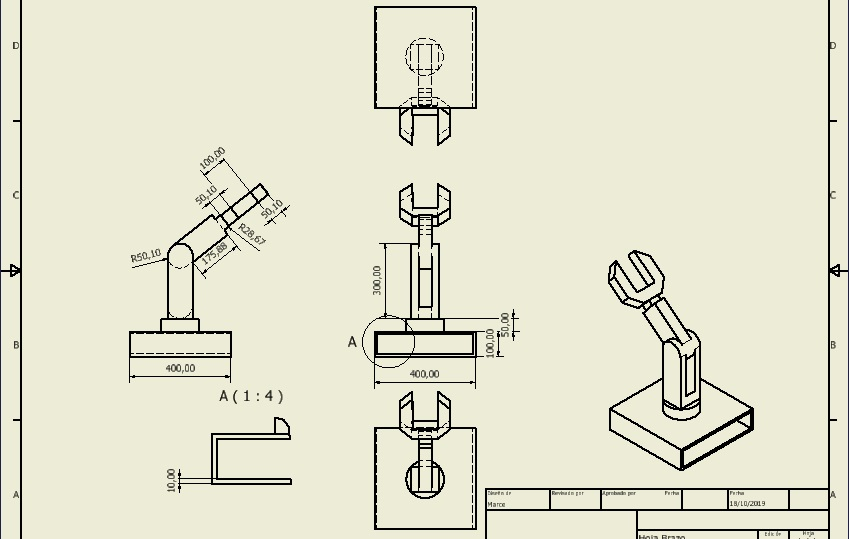
\includegraphics[scale=0.5]{Img/Hojabrazo.jpg}
     %       \caption{Medidas aproximadas y dibujo en mm}
      %      \label{fig:zo}
       % \end{figure}
    \begin{LARGE}
    \end{LARGE}
\end{large}
 Nota: las medidas mostradas se encuentran en milímetros.\\
\newpage
    \begin{thebibliography}{x}
        \bibitem{MotPas} \textsc{Anónimo} \textit{"Motor a paso."} Recuperado de:\\ 
        $https://es.wikipedia.org/wiki/Motor\_paso\_a\_paso$\\
        \bibitem{FueCon} \textsc{Fuentes conmutadas.} Recuperado de:\\
        $https://www.electronicafacil.net/tutoriales/Fuentes-conmutadas.html$


\end{thebibliography}
\end{document}






